\chapter{Substrate}

\section{Architecture}
\subsection{Guiding Principles}

Substrate aims to adhere to a few guiding principles:
\begin{enumerate}
\item Performance is flexibility. This holds true for both software and hardware.
\item Good APIs allow you to be lazy.
\item Methodology as a library. Substrate aims to be unopinionated about how you design and lay out your circuits.
  Frameworks that more rigidly prescribes how circuits are designed (eg. a library for strictly gridded layout)
  can be written as libraries using the lower-level primitives in Substrate.
  Substrate PDK plugins, for example, are simply libraries that implement a set of required functions.
  Substrate itself is a library, which means that it can be used in any Rust project or library by simply adding it to a Rust project's dependency list. Consequently, there is no such thing as a ``Substrate workspace.''
\end{enumerate}

\subsection{Contexts}

Substrate holds all state in a data structure called a \textbf{context}.
The context caches circuits that have been generated, and stores a handle to plugins (eg. for simulation or LVS) that have been initialized.
The context is thread safe and internally synchronized, so users can run multiple Substrate generators in parallel.

\subsection{Components}

The primary building block in Substrate is a \textbf{component}.
Substrate components are analogous to ``cells'' or ``modules'' in other design systems.
Components accept a set of parameters, and produce zero or more \textbf{views}.
Substrate currently supports schematic, layout, and timing views,
though other views will likely be added in the future.

In the Rust language, a type is considered a component if it implements the \verb|Component| trait shown below:

\begin{minted}{rust}
pub trait Component: Any {
    type Params: Serialize;
    fn new(params: &Self::Params, ctx: &SubstrateCtx) -> Result<Self>
    where
        Self: Sized;
    fn name(&self) -> ArcStr {
        // ...
    }
    fn schematic(&self, ctx: &mut SchematicCtx) -> Result<()> {
        // ...
    }
    fn layout(&self, ctx: &mut LayoutCtx) -> Result<()> {
        // ...
    }
}
\end{minted}

Components can contain instances of other components.

Substrate can perform the following operations on components:
\begin{itemize}
\item Export a schematic to a SPICE netlist
\item Export a layout to GDS.
\item Run LVS, DRC, or PEX, if an appropriate tool plugin is installed.
\end{itemize}

\subsection{Testbenches}
All testbenches are components with schematic views. This schematic view should be used to instantiate voltage sources and the block being simulated.

Testbenches must also implement the \verb|Testbench| trait, which provides hooks for:
\begin{itemize}
\item Setting up simulator analyses
\item Including external libraries, if necessary
\item Processing simulator output data
\end{itemize}

Substrate testbenches are expected to provide the name of their ground net.
Prior to simulation, Substrate will connect this net to the global ground net of the simulator (typically node \verb|0|).

\subsection{Process Development Kits} \label{sec:pdks}

Process development kits (PDKs) are ordinary Rust libraries that provide a type implementing the \verb|Pdk| trait shown below:

\begin{minted}{rust}
pub trait Pdk {
    fn name(&self) -> &'static str;
    fn process(&self) -> &'static str;
    fn lengths(&self) -> Units;
    fn voltages(&self) -> SiPrefix;
    fn layers(&self) -> Layers;
    fn supplies(&self) -> Supplies;
    /// Retrieves the list of MOSFETs available in this PDK.
    fn mos_devices(&self) -> Vec<MosSpec>;
    /// Provide the SPICE netlist for a MOSFET with the given parameters.
    ///
    /// The drain, gate, source, and body ports are named
    /// \verb|d|, \verb|g|, \verb|s|, and \verb|b|, respectively.
    fn mos_schematic(&self, ctx: &mut SchematicCtx, params: &MosParams) -> Result<()>;
    /// Draws MOSFETs with the given parameters
    fn mos_layout(&self, ctx: &mut LayoutCtx, params: &LayoutMosParams) -> Result<()>;
    /// Draws a via with the given params in the given context.
    fn via_layout(&self, ctx: &mut LayoutCtx, params: &ViaParams) -> Result<()>;
    /// The grid on which all layout geometry must lie.
    fn layout_grid(&self) -> i64;
    /// Called before running simulations.
    ///
    /// Allows the PDK to include model libraries, configure simulation
    /// options, and/or write relevant files.
    fn pre_sim(&self, _ctx: &mut PreSimCtx) -> Result<()> {
        Ok(())
    }
    /// Returns data that should be prepended to generated netlists,
    /// depending on the netlist purpose and the process corner.
    fn includes(&self, purpose: NetlistPurpose) -> Result<IncludeBundle> {
        Ok(Default::default())
    }
    /// Returns a database of the standard cell libraries available in the PDK.
    fn standard_cells(&self) -> Result<StdCellDb> {
        Ok(StdCellDb::new())
    }
    /// Returns a database of the available process corners.
    fn corners(&self) -> Result<CornerDb> {
        Ok(CornerDb::new())
    }
}
\end{minted}

The \verb|layers| function returns a layer database, which includes information on GDS layer numbers, layer purposes, and additional metadata (eg. identifying which metal/via layers and providing layer names).
The \verb|standard_cells| provides zero or more standard cell libraries. The standard cell API is described further in TODO.
The \verb|corners| function provides zero or more process corners. Depending on the corner the user selects, the PDK can include a different set of model libraries.
The \verb|mos_schematic| and \verb|mos_layout| functions instantiate PDK-specific CMOS devices in schematic and layout mode, respectively.
For further information on the other functions available, see the Substrate documentation.

Since PDKs are simply libraries, they are free to provide functions other than the ones specified here.
For instance, a PDK may export a component for a unit capacitor, even though Substrate currently does not
have a unified API for creating capacitors.

\section{Schematic Entry}

A very simple schematic generator, which produces an ideal resistive voltage divider, is shown below:

\begin{minted}{rust}
impl Component for VDivider {
    // ...
    
  fn schematic(&self, ctx: &mut SchematicCtx) -> Result<()> {
      let out = ctx.port("out", Direction::Output);
      let vdd = ctx.port("vdd", Direction::InOut);
      let vss = ctx.port("vss", Direction::InOut);

      ctx.instantiate::<Resistor>(&SiValue::new(2, SiPrefix::Kilo))?
          .with_connections([("p", vdd), ("n", out)])
          .named("R1")
          .add_to(ctx);

      ctx.instantiate::<Resistor>(&SiValue::new(1, SiPrefix::Kilo))?
          .with_connections([("p", out), ("n", vss)])
          .named("R2")
          .add_to(ctx);
      Ok(())
  }
}
\end{minted}

This starts by declaring three ports: \verb|out|, \verb|vdd|, and \verb|vss|, with the specified directions.
We then instantiate 2 resistors: one with value $\SI{2}{\kilo\ohm}$, and one with value $\SI{1}{\kilo\ohm}$,
and connect them appropriately.

This schematic can easily be exported to a SPICE netlist:

\begin{minted}{rust}
ctx.write_schematic_to_file::<VDivider>(&NoParams, path);
\end{minted}

Netlist generation in Substrate involves several passes:
\begin{enumerate}
\item Netlists are preprocessed to resolve duplicate net, instance, or module names.
\item The netlist is validated for correctness. This currently involves 3 analyses:
\begin{enumerate}
  \item A name-validity analysis checks for duplicate or SPICE-incompatible names.
  \item A netlist connectivity analysis verifies that all modules have their ports connected and that all widths are matched.
  \item A net driver analysis verifies that all input ports are driven by at least one source and produces warnings if nets have multiple drivers.
\end{enumerate}
\item A netlisting plugin maps the in-memory representation of Substrate components to simulator specific syntax and writes the content of the netlist to an output stream (usually a file).
\end{enumerate}

\section{Layout Entry} \label{sec:layout-entry}

Most analog generators, Substrate included, produce layouts in roughly three steps:
\begin{enumerate}
\item Generate or import sub-components.
\item Place sub-components.
\item Route between sub-components.
\end{enumerate}

The first step is described in more detail in \ref{sec:subcomponent-layout-generation},
the second step in \ref{sec:placement-utilities}, and the third in \ref{sec:routing}.

\subsection{Subcomponent Layout Generation} \label{sec:subcomponent-layout-generation}

This section describes how base-layer components, such as transistors, resistors, and capacitors, can be generated or imported into Substrate.

\subsubsection{Hard Macros} \label{sec:hard-macros}
Hard macros allow users to import arbitrary layouts into Substrate, and use them as if they were regular components. They are useful when you are incorporating externally-provided cells (eg. provided by a foundry or generated by a tool other than Substrate), or where writing generator code would be slower and have little benefit over a hand-drawn layout.

Hard macros can be incorporated into Substrate using the \verb|hard_macro| attribute, which is a Rust procedural macro.

\begin{minted}{rust}
#[hard_macro(
    name = "sram_sp_cell",
    pdk = "sky130-open",
    path_fn = "path",
    gds_cell_name = "sky130_fd_bd_sram__sram_sp_cell_opt1",
    spice_subckt_name = "sram_sp_cell"
)]
pub struct SpCell;
\end{minted}

The arguments to the procedural macro allow the user to specify a path function. The path function accepts a single argument – a view type (ie. schematic or layout) – and returns the path at which the appropriate view is stored (ie. a SPICE netlist or a GDS file, respectively).

Hard macros can then be instantiated as regular Substrate components, in both layout and schematic mode:
\begin{minted}{rust}
ctx.instantiate::<SpCell>(&NoParams);
\end{minted}

\subsubsection{Raw Layout Utilities}

In the spirit of giving the user complete control over generated layout, Substrate allows users to
specify layouts down to individual polygons. To create layout geometry, users specify a layer
(obtained from the PDK API described in \ref{sec:pdks}) and a shape.

There is a rich system of utilities for manipulating rectangular geometry, since rectangles are the
predominant shape in integrated circuit layouts. The Substrate documentation lists the full set of
helpers; an image of one page of the documentation is included here for reference.

\begin{figure}[htb] \centering
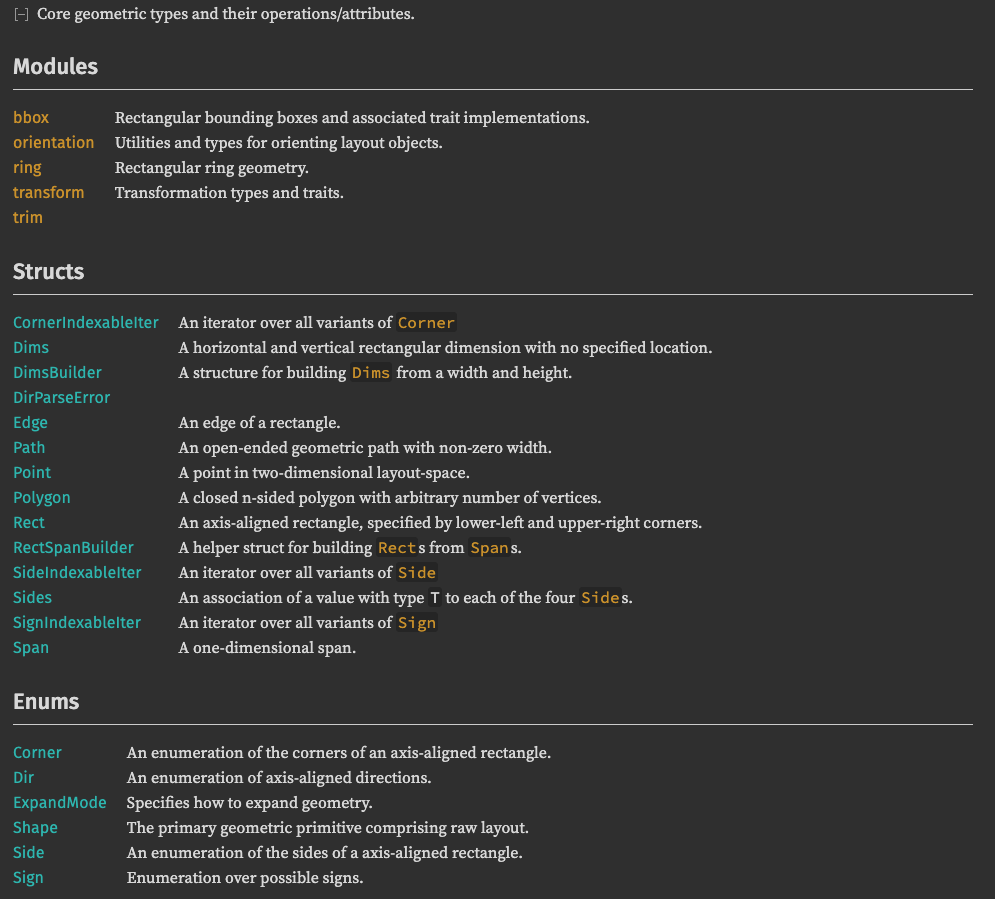
\includegraphics[width=0.8\textwidth]{figures/subgeom.png}
\caption{
    An example page taken from Substrate's geometry API documentation.
}
\end{figure}


The raw layout system provides utilities for:
\begin{itemize}
\item Creating and resizing rectangles.
\item Grouping layout elements (such as rectangles and instances of subcomponents).
\item Relative placement/alignment of layout elements.
\item Rotating/mirroring layout elements and groups of layout elements.
\item Calculating bounding boxes.
\item Flattening hierarchical layout elements.
\item Trimming geometry that lies outside a masking shape.
\end{itemize}

\subsubsection{PDK-provided Unit Cells}

\subsection{Placement Utilities} \label{sec:placement-utilities}

The basis for all placement utilities in Substrate is the \verb|AlignRect| trait,
which provides functions for rectangular/Manhattan positioning for types
that are translatable and have a bounding box.

Users of the \verb|AlignRect| trait specify an \verb|AlignMode|, a reference bounding box or rectangle,
and a spacing. The implementation of the \verb|AlignRect| trait then performs the computations to place
a new bounding box at the requested position relative to the reference box.

The \verb|AlignMode| trait is shown below.

\begin{minted}{rust}
pub enum AlignMode {
    Left,
    Right,
    Bottom,
    Top,
    CenterHorizontal,
    CenterVertical,
    ToTheRight,
    ToTheLeft,
    Beneath,
    Above,
}
\end{minted}

These options generally do what you expect. For example, \verb|AlignMode::Right| aligns the right edges of two boxes,
whereas \verb|AlignMode::ToTheRight| aligns one box to the right of another box.
If a spacing is specified, \verb|AlignMode::ToTheRight| aligns the second box to the right of the first box,
while leaving the desired spacing in between.

Although the alignment API can be directly useful,
it is often more convenient to use higher-level abstractions
when describing the layout of regular (eg. gridded) structures.
To this end, Substrate provides a variety of tiling APIs.

Each of Substrate's tiling implementations takes as input one or more tiles,
as well as metadata about how to place those tiles:
\begin{itemize}
\item The \verb|ArrayTiler| takes a list of tiles, and places them in a vertical or horizontal line.
\item The \verb|GridTiler| takes a 2D array of tiles, and places them in a grid.
\item The nine patch tiler \verb|NpTiler| takes 9 tiles, and two numbers, $n_x$ and $n_y$.
  It tiles these 9 tiles in a manner similar to nine patch images.
  The center tile is repeated in an $n_x \times n_y$ grid.
  The top and bottom edge tiles are repeated in an $n_x \times 1$ array
  directly above and below the center tile grid, respectively.
  The left and right edge tiles are similarly placed in an $n_y \times 1$ array.
  The corner tiles are placed, unrepeated, at the corners of the center tile grid.
\end{itemize}

Each of these tilers uses the raw alignment API to position tiles.
To avoid silent errors, the tiling implementations check that tiles have compatible sizes.
For example, in a grid tiling instance, all tiles in the same column must have the same width,
and all tile in the same row must have the same height.

To ensure that the tiling APIs are composable, the tilers have few requirements
on what can constitute a tile: anything can be tiled, as long as it can be drawn
into a Substrate layout, and it has a bounding box.

This flexibility makes it easy to add new tile types – to mark a type as tileable,
it just needs to be marked with the \verb|CustomTile| trait (which in turn requires
the type to be drawable and have a bounding box). Indeed, Substrate uses
this flexibility internally to provide custom tile types of its own.

For example, it is common to tile objects according to their bounding box
on a specific layer (rather than their overall bounding box).
Tiling standard cells is a common example in which this problem arises.
In Substrate, supporting layer-specific bounding box tiling requires no changes
to the tiler implementation at all.
Instead, Substrate provides the \verb|LayerBbox| tile type, which implements the
aforementioned \verb|CustomTile| trait. The \verb|LayerBbox| constructor takes an inner tile
(eg. a standard cell layout) and a layer identifier, and exposes a standard tile API to the tiler:
\begin{itemize}
\item Drawing a \verb|LayerBbox| tile simply results in drawing the inner tile.
\item When calculating the bounding box, \verb|LayerBbox| filters the elements of the inner tile, considering
  only the elements on its selected layer.
\end{itemize}

Similarly, there is a \verb|Pad| tile type, which adds padding to an inner tile as follows:
\begin{itemize}
\item Drawing the \verb|Pad| tile simply draws the inner tile.
\item The bounding box of the \verb|Pad| tile is the bounding box of the inner tile, expanded by the width of the padding.
\end{itemize}

These custom types are easily composable. For example, you can create a \verb|Pad| tile that wraps a \verb|LayerBbox| tile
that in turn wraps a ``regular'' tile.


\subsection{Routing} \label{sec:routing}

There are three levels of routing abstraction in Substrate:
1. The lowest level of abstraction deals with routing tracks. This layer provides utilities for calculating
   track locations, locating tracks near a point, and creating half tracks
   (tracks that are half the width of a normal track, with the expectation that two half tracks will abut
   to form a full-size track).
2. The second level of abstraction handles manual routing. This layer is intended for situations in which
   routing performance is important and the rough shape of the route is known in advance. One such situation is
   routing the output of a standard cell inverter to the input of an adjacent inverter. This layer
   provides methods for creating elbow jogs, S-shaped jogs, and collections of multiple parallel jogs.
3. The third and highest level of abstraction is fully automatic gridded routing. Users define a routing grid,
   then request that the router draw routes. Each routing request contains a source location and layer,
   a destination location and layer, and a net name string. Reusing a net name across multiple routing requests
   enables the router to reuse routes previously drawn on that net. The algorithm currently used for routing
   is essentially breadth-first search; the router does not attempt to find globally optimal routes.

Further examples of the routing APIs are given later in this thesis, in the context of SRAM22.

